
\documentclass{article}
\usepackage{tikz}
\usetikzlibrary{patterns}
\usepackage{graphicx} 
\usepackage{subfigure}
\usepackage{mathpazo}
\usepackage{pgfplots}
\newcommand*{\num}{pi}

\graphicspath{ {C:/Users/Jacki/Pictures/} }
\begin{document}

\begin{figure}
\center
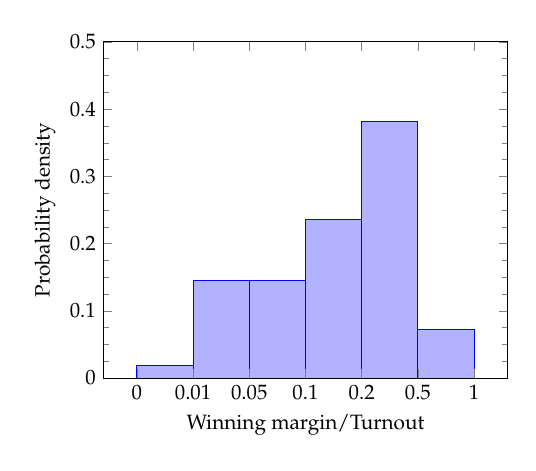
\begin{tikzpicture}[scale=0.75]
\begin{axis}[
    ylabel = Probability density,
    xlabel = Winning margin/Turnout,
    ymin=0, ymax=0.5,
    minor y tick num = 3,
    area style,
	xtick={0,2,4,6,8,10,12,14,16},
	xticklabels={$0$,$0$,$0.01$,$0.05$,$0.1$,$0.2$,$0.5$,$1$},
    ]
\addplot+[ybar interval,mark=no] plot coordinates { (2, 0.0182) (4, 0.145) (6, 0.145) (8, 0.236) (10, 0.3818) (12,0.0727) (14,0)};
\end{axis}
\end{tikzpicture}
\caption{90s}

\center
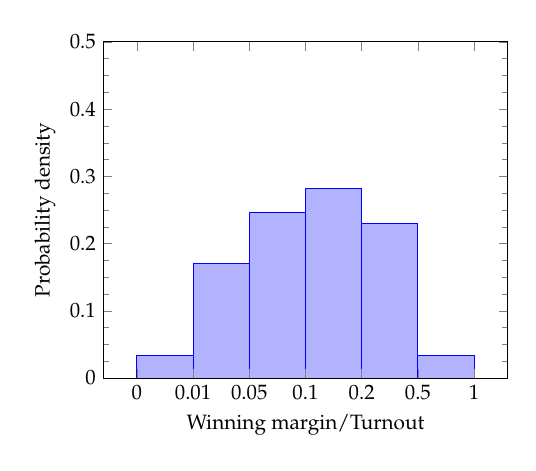
\begin{tikzpicture}[scale=0.75]
\begin{axis}[
    ylabel = Probability density,
    xlabel = Winning margin/Turnout,
    ymin=0, ymax=0.5,
    minor y tick num = 3,
    area style,
	xtick={0,2,4,6,8,10,12,14,16},
	xticklabels={$0$,$0$,$0.01$,$0.05$,$0.1$,$0.2$,$0.5$,$1$},
    ]
\addplot+[ybar interval,mark=no] plot coordinates { (2, 0.0342) (4, 0.171) (6, 0.247) (8, 0.282) (10, 0.2307) (12,0.03418) (14,0)};
\end{axis}
\end{tikzpicture}
\caption{00s}

\center
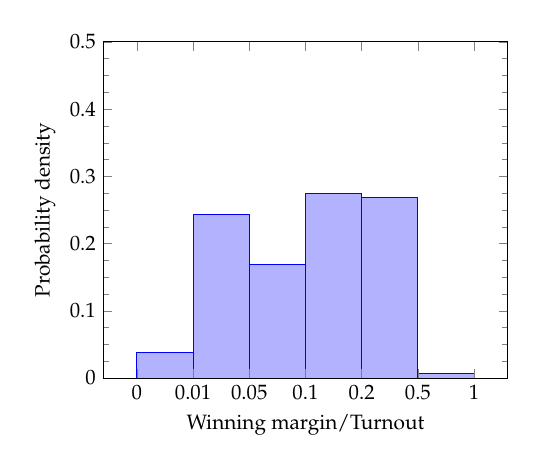
\begin{tikzpicture}[scale=0.75]
\begin{axis}[
    ylabel = Probability density,
    xlabel = Winning margin/Turnout,
    ymin=0, ymax=0.5,
    minor y tick num = 3,
    area style,
    xtick={0,2,4,6,8,10,12,14,16},
    xticklabels={$0$,$0$,$0.01$,$0.05$,$0.1$,$0.2$,$0.5$,$1$},
    ]
\addplot+[ybar interval,mark=no] plot coordinates { (2, 0.0375) (4, 0.24375) (6, 0.16875) (8, 0.275) (10, 0.26875) (12,0.00625) (14,0)};
\end{axis}
\end{tikzpicture}
\caption{10s}
\end{figure}

\end{document}